\documentclass[12pt,notitlepage]{amsart}
\usepackage{inputenc}
\usepackage[margin = 1in]{geometry}
\usepackage{ragged2e}
\geometry{letterpaper}
\usepackage{cite}
\usepackage{graphicx}
\usepackage{setspace}
\usepackage{amssymb}
\usepackage{epstopdf}
\usepackage{tikz}
\usetikzlibrary{shapes,arrows}
\usepackage{booktabs}% http://ctan.org/pkg/booktabs
\newcommand{\tabitem}{~~\llap{\textbullet}~~}
\DeclareGraphicsRule{.tif}{png}{.png}{`convert #1 `dirname #1`/`basename #1 .tif`.png}
\graphicspath{
    {Pics/PDFs/}
    {Pics/JPGs/}
    {Pics/PNGs/}
}
%add description of MeOH bath... explain why the search for better method. describe math of how density changes the time. Describe heat tranfer.
\begin{document}
\onehalfspacing
  \tikzstyle{block} = [rectangle, draw, fill=blue!20, 
    text width=2cm, text centered, rounded corners, minimum height=2cm]
\tikzstyle{line} = [draw, -latex']


 \begin{titlepage}
   \begin{center}
       \vspace*{1cm}
 
       \textbf{Slow Solidification of Ammonia for Polarized Targets}
 
       \vspace{0.5cm}
        something awesome
 
       \vspace{1.5cm}
 
       \textbf{Lucas Jameson}
 
       \vfill
 
       A thesis presented for the degree of\\
       Bachelors of Science
 
       \vspace{0.8cm}
 
%       \includegraphics[width=0.4\textwidth]{university}
 
       Department of Physics\\
	   University of New Hampshire\\
       United States of America\\
       May 18, 2019
 
   \end{center}
\end{titlepage}
\newpage
\begin{abstract}
Polarized targets are produced at Slifer Lab as part of the New Hampshire (UNH) Nuclear Physics Group (NPG)  research program. The goal is to produce polarized targets with a Dynamic Nuclear Polarizer (DNP) that is used in the spin-dependent physics program at Jefferson Lab. Ammonia that has free radicals by irradiation and is polarized by Dynamic Nuclear Polarization is a common polarized target. A new method for solidifying ammonia was implemented with the intent of producing higher density solid ammonia. This method utilized a solid copper rod mounted to the bottom of the solidification chamber that pulled heat from the chamber and sank it in a bath of liquid nitrogen. This allowed for the chamber walls to get to a temperature that was closer to the freezing point of ammonia and allowed it to solidify in a slower manner and increased the density. The measurement of the density of the slowly frozen ammonia is in progress but qualitative analysis supports the material will have a higher density. 
\end{abstract}

\newpage
  \tableofcontents
\newpage
 
  \section{Introduction}
Polarized targets are produced at Slifer Lab as part of the University of New Hampshire (UNH) Nuclear Physics Group (NPG) research program. The goal is to produce polarized targets with a Dynamic Nuclear Polarizer (DNP) that is used in the spin-dependent physics program at Jefferson Lab. Ammonia that has free radicals introduced by irradiation and is polarized by Dynamic Nuclear Polarization is a common polarized target since it has (state why its so common). The ammonia made using the current method of a liquid nitrogen bath made a porous solid material that was easy to break and was relatively low in density.  A new method for solidifying ammonia was implemented with the intent of producing higher density solid ammonia. The reason for creating a new method for producing solid ammonia with higher density was to shorten the time scale needed to run the scattering experiment. The measurable differential cross section into some area of the scattering experiment is given by \cite{nuke}
\begin{equation}
\frac{d\sigma}{d\Omega} = \frac{N}{\mathcal{L}t}
\end{equation}
Since the uncertainty of the counts is
\begin{equation}
\delta N = \frac{1}{\sqrt{N}}
\end{equation}
and  $\frac{d\sigma}{d\Omega} $ should not change with the change in target density but the experiment run time \cite{maxwell}
\begin{equation}
t = \frac{1}{fP^{2} \mathcal{L} N_{t} \Delta A^{2}}
\end{equation}
will decrease as the scattering centers increases, this allows the time the experiment can run for to be increased. With increased experiment run time the number of scattered particles increases leading to a small uncertainty in the measured counts. 
$N$ is the counts measured, $t$ is the time the experiment runs for,  and $\mathcal{L} = \phi_{b} n_{b}Ad$, $\phi_{b}$ is the beam current and $Ad$ accounts for the geometric properties of the target. The goal is to increase the target density $n_{b}$ holding everything else fixed. This method utilized a solid copper rod mounted to the bottom of the cryostat that pulled heat and sank it in a bath of liquid nitrogen. This allowed for the chamber walls to get to $188$ K that was closer to the freezing point of ammonia which is $195$ K and allowed it to solidify in a slower manner taking $5$ hours to fill half the cryostat. The processed made roughly $120$ mL of material and increased the density. The slow freezing method allows the ammonia to liquefy first and since the bottom is the coldest part, the crystal begins to form from the bottom up.  The measurement of the density of the slowly frozen ammonia is in progress and current qualitative analysis supports the fact that the material will have a higher density. 
  
  
  
  \subsection{Polarized Targets in Nuclear Physics}  In order to study the spin structure of the proton a polarized electron beam is scattered off a polarized target through inclusive Deep Inelastic scattering.
  The differential cross section for this process is given as \cite{maxwell,nuke,ellie},
  \begin{equation}
  \frac{d\sigma}{d\Omega•} = \frac{\alpha}{Q^{4}} l_{\mu \nu}W^{\mu \nu}
  \end{equation}
  where 
  \begin{equation}
  W^{\mu \nu} = \alpha F_{1}(Q^{2}) + \beta F_{2}(Q^{2}) + i \gamma g_{1}(Q^{2}) + i \delta g_{2}(Q^{2}) 
  \end{equation}
  by running the experiment twice, once with the beam polarization aligned with the target polarization and again with the beam polarization anti-aligned with the target polarization,
  the difference in the differential cross section is defined as 
     \begin{equation}
   \sigma_{ll} = \frac{1}{2}(\sigma_{\Uparrow}^{\Uparrow} - \sigma_{\Uparrow}^{\Downarrow})
   \end{equation}
  and a change into units of Bjorken x and y where 
  \begin{eqnarray}
  x = \frac{Q^{2}}{2m_{p}\nu} ,&
  y = 1 - \frac{E'}{E}
  \end{eqnarray}
  make the expression easier to work with. Physically Bjorken x is a scaling variable that scales the measurements to the mass of the target. Therefore a proton will land at $x=1$ and the mass of the nuclei will land at $x = A$. Bjorken y physically is how much energy is deposited to the scattered particles. The doubly differential cross section is redefined in terms of Bjorken x and the 4-momentum transfer and eliminates the structure functions $F_{1}, F_{1}$. 
    \begin{equation}
  \frac{d\sigma_{ll}}{dQ^{2}dx•} = \frac{8\pi\alpha^{2}\hbar^{2}y}{Q^{4}} \big[\big(1- \frac{y}{2} - \frac{yxMc^{2}}{2E}\big) g_{1}(x,Q^{2}) - \frac{xMc^{2}}{E}g_{2}(x,Q^{2})\big]
   \end{equation}
  
   
\begin{figure}[h]
\caption{Schematic of a generic scattering experiment using polarized targets.}
\label{scatter}
\centering
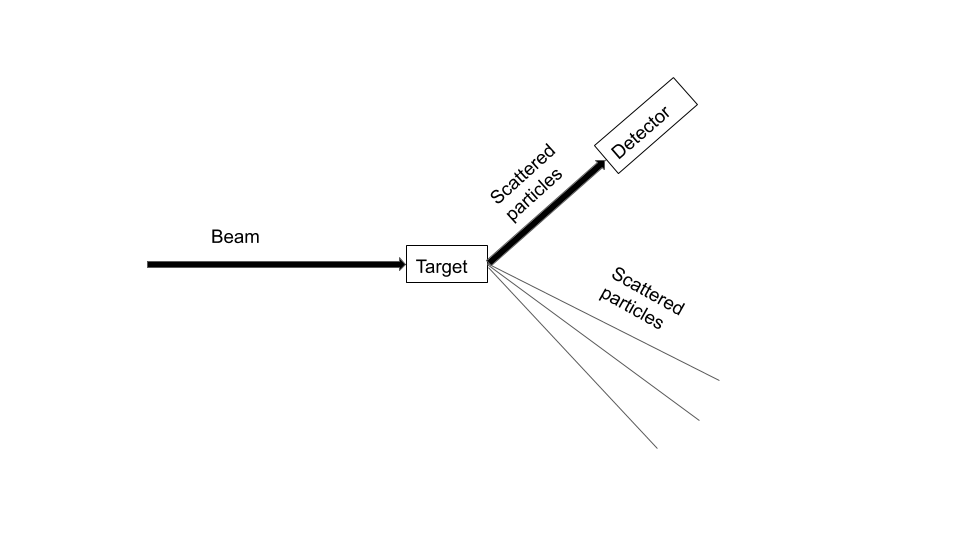
\includegraphics[width = 10cm,height = 6cm]{Scattering_exp} 
\end{figure}

  \subsection{Production of Polarized Targets at UNH}  The UNH NPG research program produces polarized targets by creating proton rich solids that are doped with free electron radicals \cite{mellor}. The material is submerged in a strong magnetic field of about $5$ T and low temperature around $1$ K and by using mm-wave microwaves to induce a spin flip of the electron and carry a proton spin flip along with in order to conserve total angular momentum of the system as shown in Figure \ref{DNPprocess}. 
\begin{figure}[h]
\caption{Schematic of the DNP process the DNP system uses.}
\label{DNPprocess}
\centering
\includegraphics[width = 8cm,height = 6cm]{DNPprocess} 
\end{figure}
 
 
Over a period of $~30$ min the sample of ammonia will become polarized up to $~90\%$.  Other material like TEMPO doped butyl alcohol and TEMPO doped epoxy are also common targets. Ammonia is a good target material due to its radiation hardness, large polarization, and the spin decay rate is small compared to other target material. (Fact check) \cite{karl}  
\begin{figure}[h]
\label{procedure}
\begin{tikzpicture}[node distance = 4cm, auto]
    % Place nodes
    \node [block] (freeze) {Solidify ammonia using gas panel};
    \node [block, right of=freeze] (crush) {Crush the material into $~2$ mm beads};  
    \node [block, right of=crush] (store) {Store material in liquid nitorgen};    
    \node [block, right of=store] (irad) {Irradiate the material at NIST};        
    \node [block, below of=irad] (pol) {Polarize the material using DNP};    
    % Draw edges
    \path [line]  (freeze) -- (crush) ;
    \path [line]  (crush) -- (store) ;
    \path [line]  (store) -- (irad);
    \path [line] (irad) -- (pol);
\end{tikzpicture}
\end{figure}  
The polarized target production process starts with the production of solid electronics grade ammonia that is produced using the gas panel shown in Figure \ref{gaspanel}.
\begin{figure}[ht]
\caption{Schematic of the device to measure the density.}
\label{gaspanel}
\centering
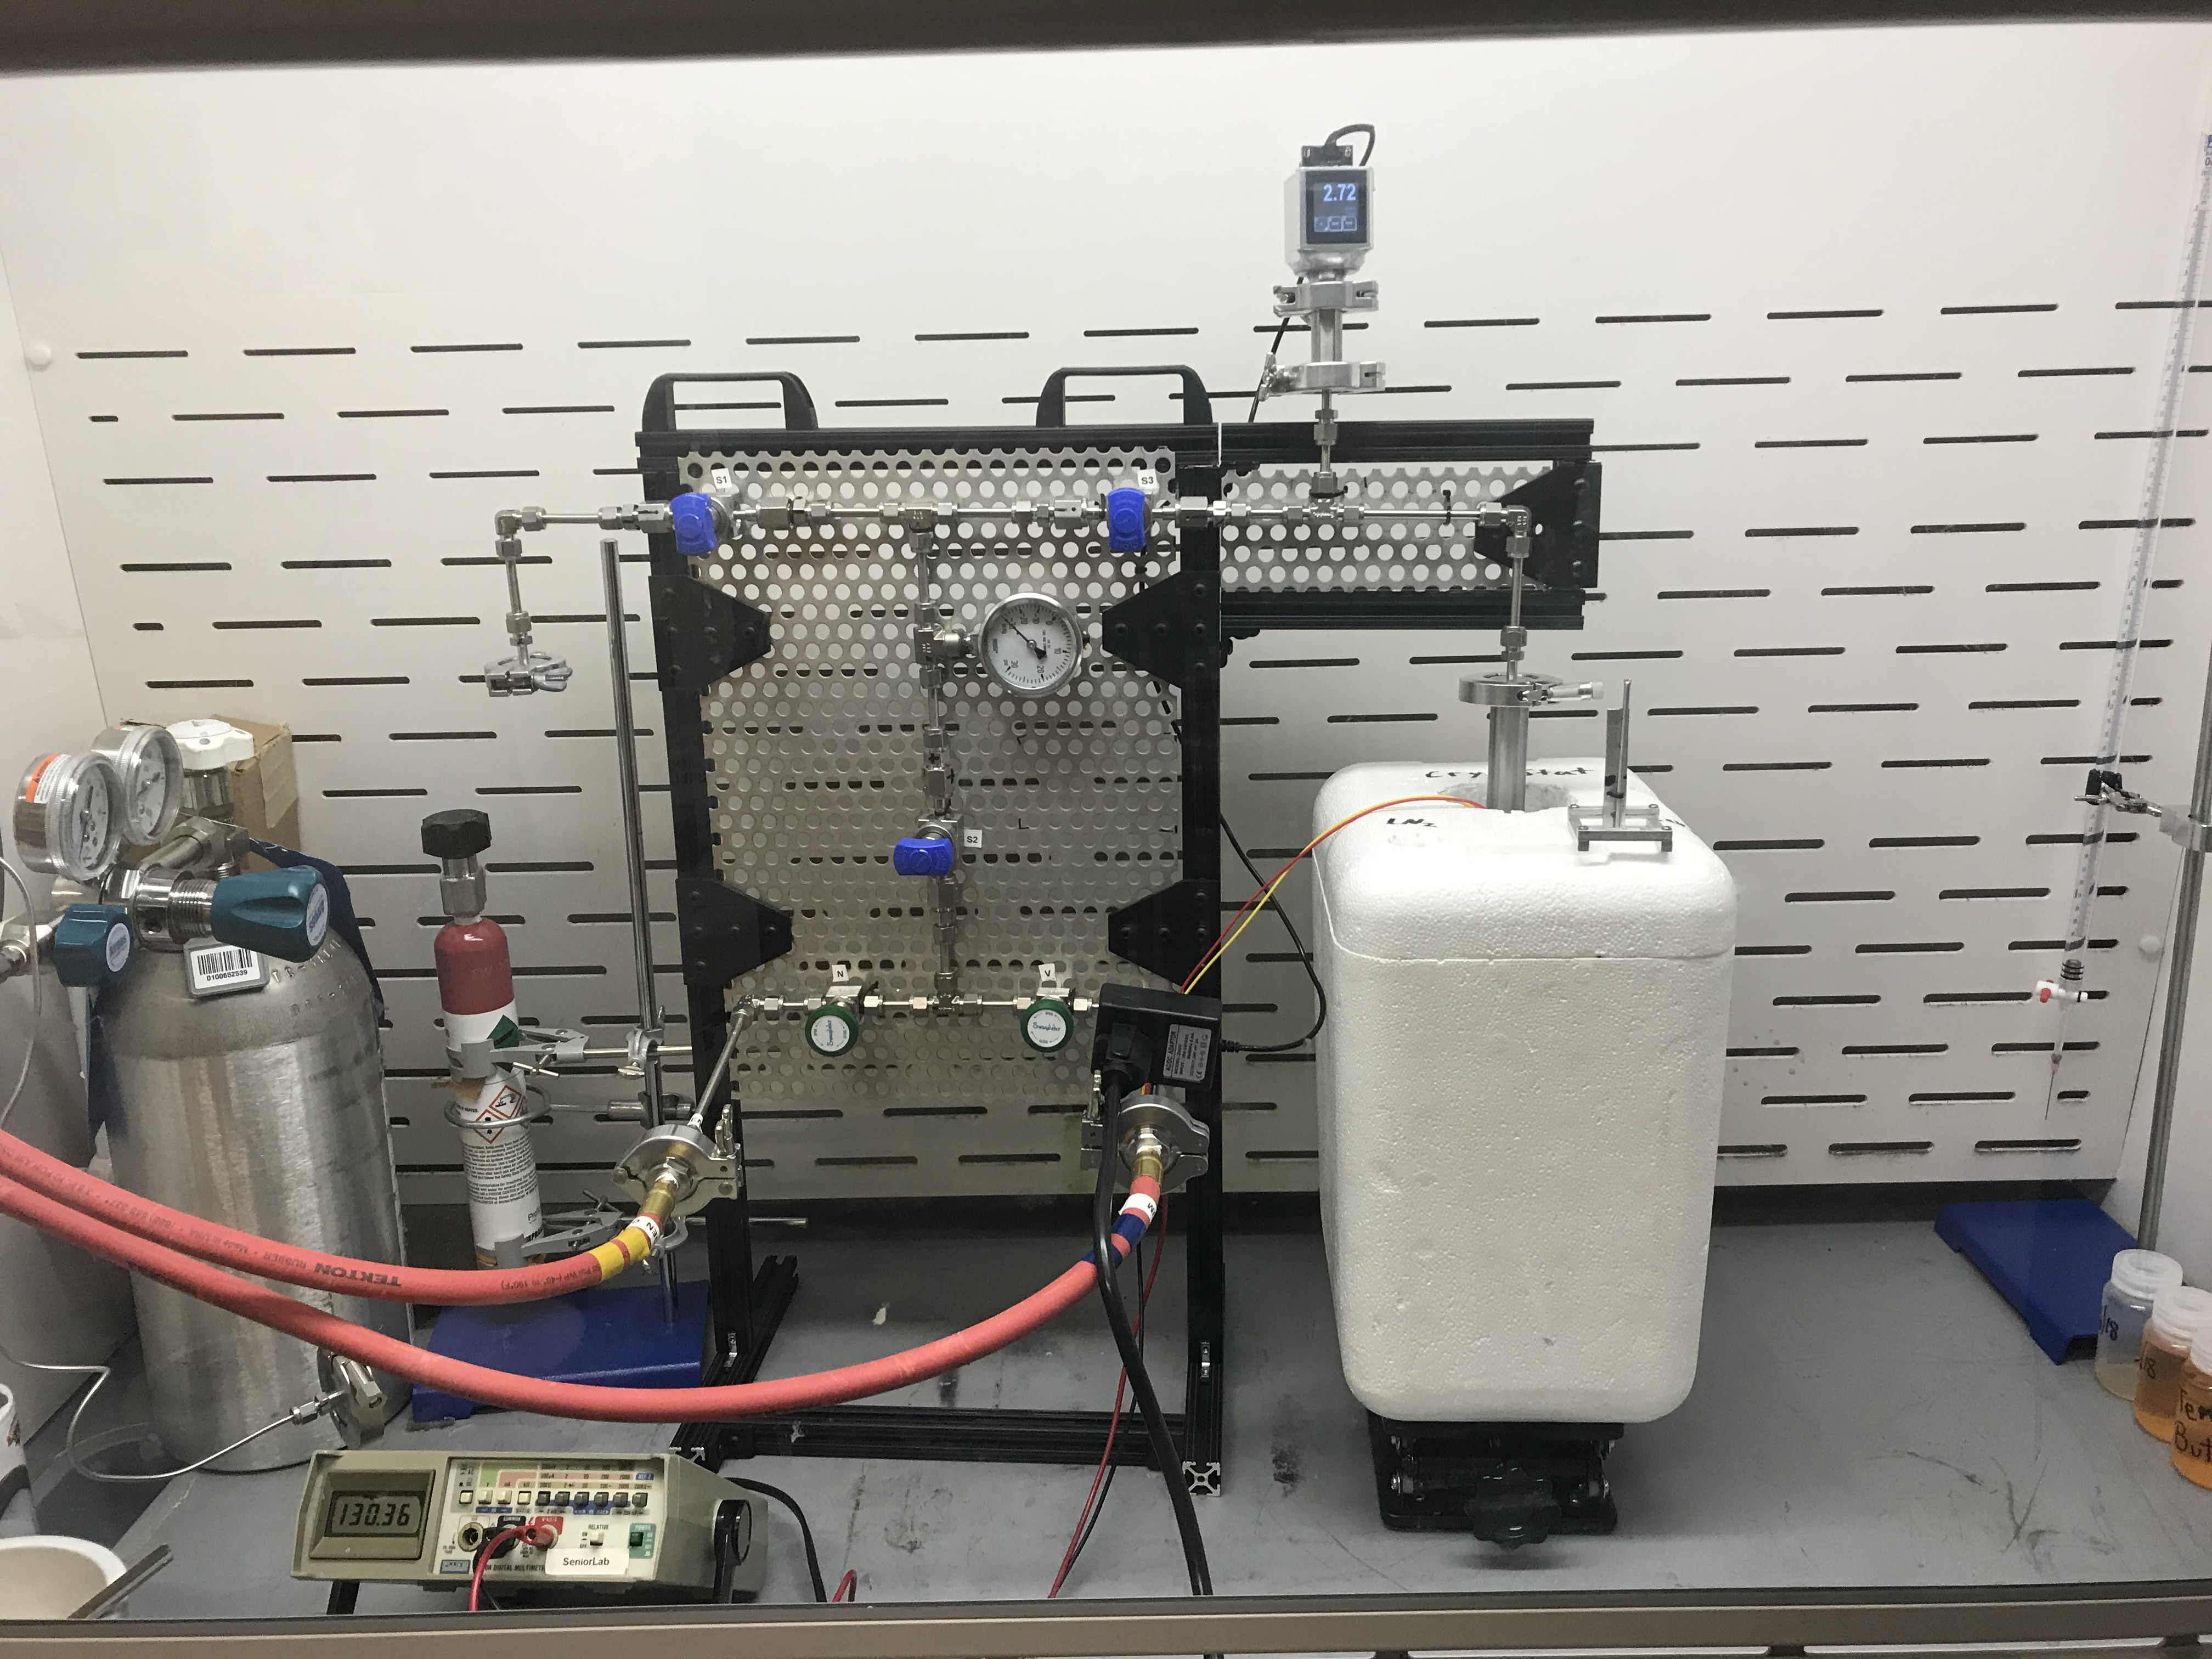
\includegraphics[width = 8cm,height = 6cm]{Gas_Panel} 
\end{figure}
Once the material is frozen and harvested, it is sorted into $2$ mm beads using the apparatus shown in Figure \ref{Crusher}. 


 \begin{figure}[ht]
\caption{The device used to sort the material into $2$ mm beads.}
\label{Crusher}
\centering
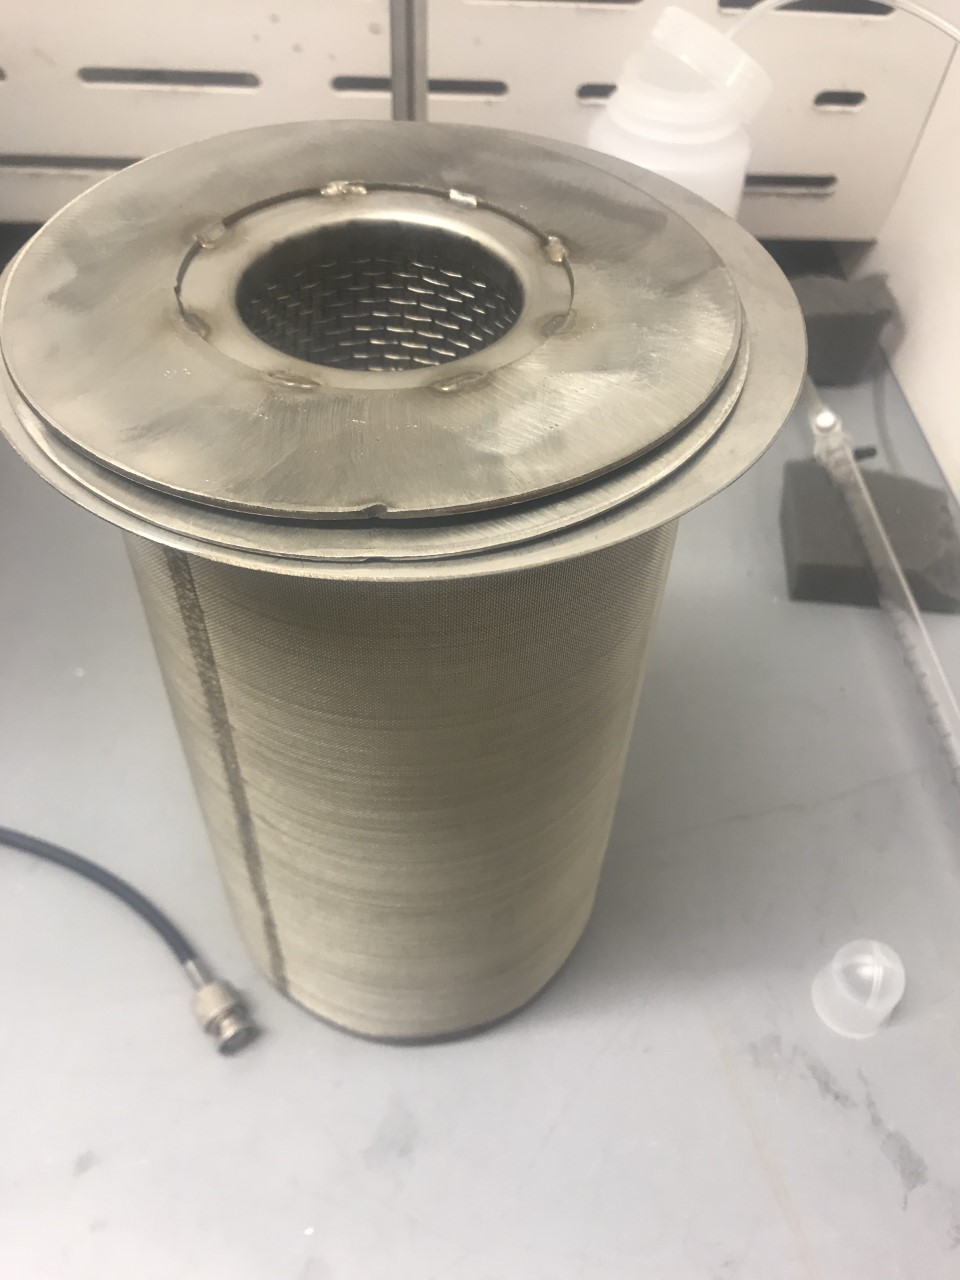
\includegraphics[width = 6cm,height = 8cm]{Crusher} 
\end{figure}


The sorted material is then irradiated at National Institute of Science and Technology(NIST) with the optimal dose that is to be determined to achieve maximum polarization in the material \cite{jay}.
 \begin{figure}[ht]
\caption{Plot showing how the polarization depends on the dose.}
\label{DNP}
\centering
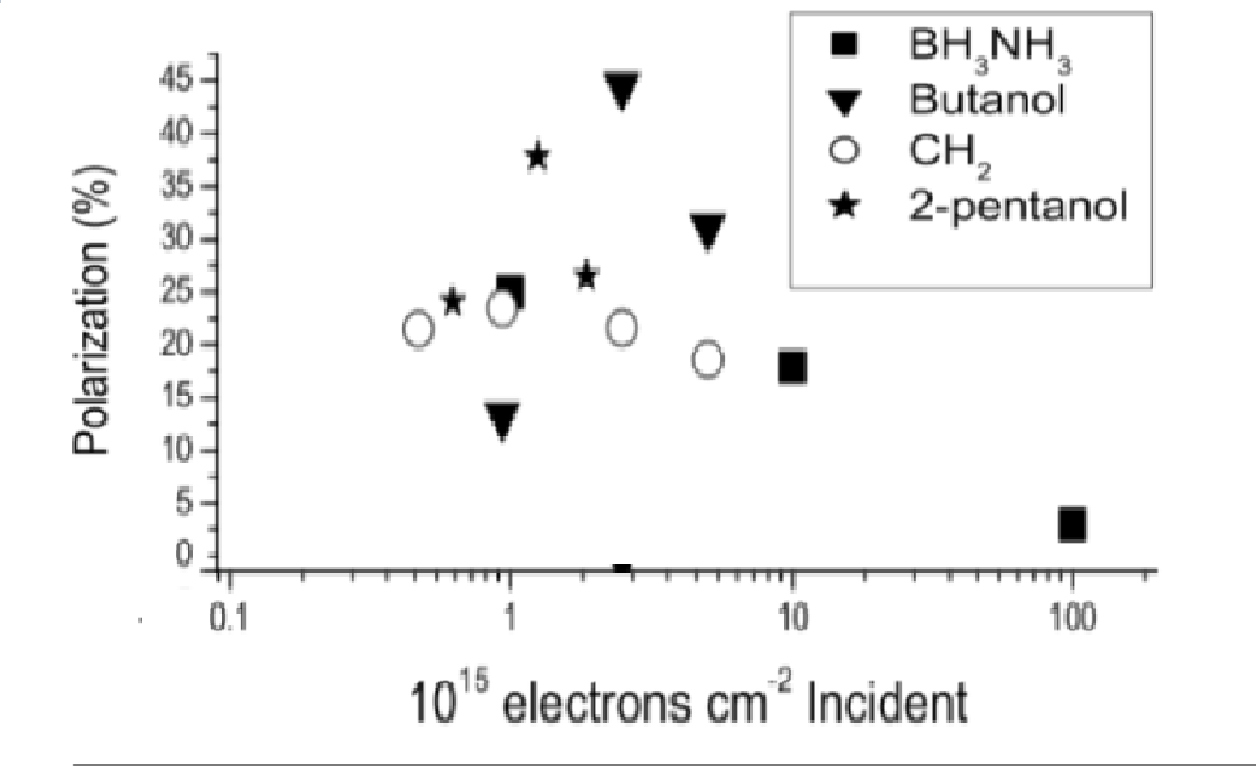
\includegraphics[width = 8cm,height = 6cm]{DoctoredData} 
\end{figure}

The irradiated material is placed in the DNP system at Slifer Lab shown in Figure \ref{DNPprocess} and is polarized. 

   \begin{figure}[ht]
\caption{Schematic of the DNP system at UNH.}
\label{DNP}
\centering
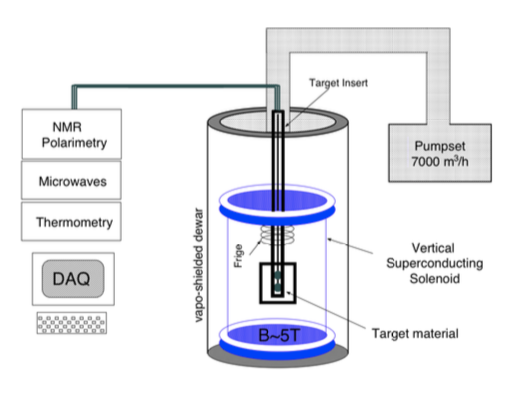
\includegraphics[width = 8cm,height = 6cm]{DNP_sys} 
\end{figure}
After that the material awaits distribution to national accelerators. 
 


 
  \section{Methods and Experimental Setup}The solidification process for ammonia initially used a liquid nitrogen bath in which the internal walls of the cryostat got well below the melting point of ammonia which resulted in the material solidifying at a much faster rate and producing more material. The new process involves solidifying the material at a slower rate using a temperature closer to the melting point of ammonia. This allows the solid to grow from the bottom up and form a crystal structure. 
    \begin{figure}[h]
 \caption{Schematic of the device to measure the density.}
 \label{Tvt}
 \centering
  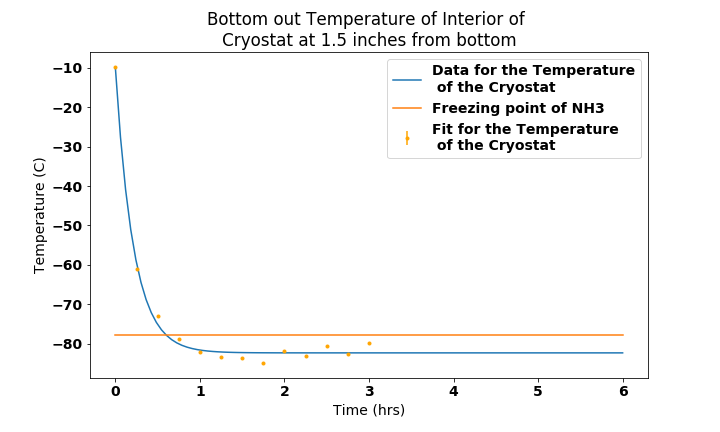
\includegraphics[width = 10cm,height = 6cm]{Temperature_Time_2}
\end{figure}

The temperature can be modeled mathematically by Fourier's law for a given material through \cite{HT}. $\alpha \equiv \frac{k_{c}}{\rho c_{p}}$ where $k_{c}$ is the thermal conductivity of the material, $\rho$ is the density, and $c_{p}$ is the specific heat. 
\begin{equation}
\frac{\partial T}{\partial t} = \alpha \nabla^{2} T.
\end{equation}
The time dependence can be isolated by separating and integrating. The temperature can then be written as 
\begin{equation}
T(\vec{r}, t) = R(\vec{r}) e^{-\lambda t}
\end{equation}
with 
$\lambda = \frac{k}{\alpha}$
and 
$R(\vec{r})$ satisfies the following 
\begin{equation}
 \nabla^{2}R(\vec{r})= -k R(\vec{r}).
\end{equation}
This provides a way to look at the time dependence of the temperature of the cryostat and given the pressure, the phase of the ammonia in the cryostat can be determined. 
\begin{figure}[h]
 \caption{Phase diagram for ammonia}
 \label{PDNH3}
 \centering
 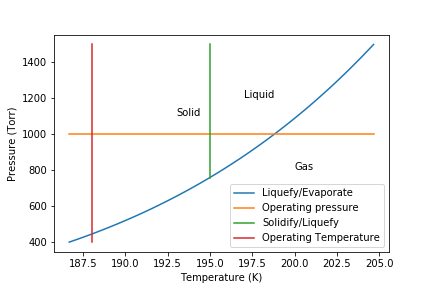
\includegraphics[width = 8cm,height = 6cm]{NH3_PD_2} 
\end{figure}
During operation of the gas panel using the coldfinger method, the cryostat has a large thermal gradient of $~50$ K due to the thermal properties of the stainless steel. The lowest temperature is $~ 193$ to $~ 180$ K and the maximum temperature at the top of the cryostat is $~ 238$ K. At an operating pressure of $~ 1000$ Torr this provides a region where most of the cryostat is able to liquefy the gaseous ammonia and a crystal can grow from the bottom. 
  
  
  
  
  \subsection{Solidification of Ammonia} 
  some cool stuff here about the different methods and why. 
  \subsubsection{Liquid Nitrogen Bath}
  Prior methods of solidifying ammonia at UNH included using a liquid nitrogen cold bath to chill the cryostat down to a temperature of much less then the melting point of ammonia. The entire cryostat is submerged in the liquid nitrogen bath and results all the walls of the cryostat cooling down to well below the melting point of ammonia. As gaseous ammonia interacts with the walls of the cryostat, the ammonia beads up on the walls and forms a solid on the wall. The solid thus grows from the walls of the cryostat inward. This process results in a faster solidification process and a material that is an amorphous and powdery solid. 
  \subsubsection{Methanol/Liquid Nitrogen Cold Bath}  
  Working towards slow solidification, a method using a methanol cold bath to cool the cryostat down to just below the melting point was developed and eventually abandoned for the coldfinger method due to the process's complexity. This method involved using a liquid nitrogen cooling helix to cool a large bath of methanol to just above the freezing point, then the cooling helix was removed and methanol ice cubes were placed in the bath to maintain a stable temperature. This method was complex and used $~20$ L of liquid nitrogen for a single solidification run. 
    \subsubsection{Coldfinger Method}
  As gaseous ammonia flows into the cryostat it deposits heat into the walls and begins to liquefy. A pool of liquid ammonia forms on the bottom of the freezing chamber first and then a solid slowly begins to grow from that. To ensure that the coldfinger is working properly, the entire copper rod must remain under liquid nitrogen. This allows the coldfinger to remain at a constant temperature and to optimize performance. After the solidification process has finished, typically several hours for half the freezing chamber to be filled, the material is harvested from the freezing chamber and crushed and sorted into $~2$ mm beads. These are then stored in $30$ mL Nalgene bottles and stored in liquid nitrogen until they get irradiated and polarized. 

The coldfinger system \cite{cf} is submerged in a bath of liquid nitrogen and acts as a heat sink to cool down the interior walls of the freezing chamber to $195$ K which is the freezing point of ammonia. The level of liquid nitrogen in which the coldfinger sits is to be maintained such that the entire copper rod is fully submerged at all times. A dewar with a level probe is used to ensure that the level of liquid nitrogen remains constant by periodically adding liquid nitrogen to the dewar.
 \subsubsection{Future Developments}
Future cooling procedure plans to create a high density solid involve revisiting the cold bath procedure but modifying the cooling apparatus for the process. By using a coldfinger apparatus attached to the bottom of a aluminum container full of $86:14$ diluted methanol by volume can get to well below the solidification temperature \cite{winans} and make the thermal gradients smaller. The dilution of methanol introduces freezing point suppression and can get to $~143$ K.  Another option is to build the cryostat out of aluminum instead of stainless steel. 


\subsection{Density Measurement of Cryogenic Solids}The density of  the material can be measured using Archimedes principle where the fluid used to measure the displaced volume is liquid nitrogen \cite{oscar}. In order to make accurate measurements on the volume of liquid nitrogen in the graduated cylinder, the whole system in placed in a rough vacuum. By pulling rough vacuum on the liquid nitrogen, the boiling point lowers and we are keeping only the cold liquid nitrogen, as the device is vented back to atmosphere, the pressure rises and the liquid nitrogen begins to heat back up. This gives $1-2$ minutes for a measurement to be made where the liquid nitrogen is stable and not boiling vigorously.
\begin{figure}[h]
 \caption{Schematic of the device to measure the density.}
 \label{rho}
 \centering
 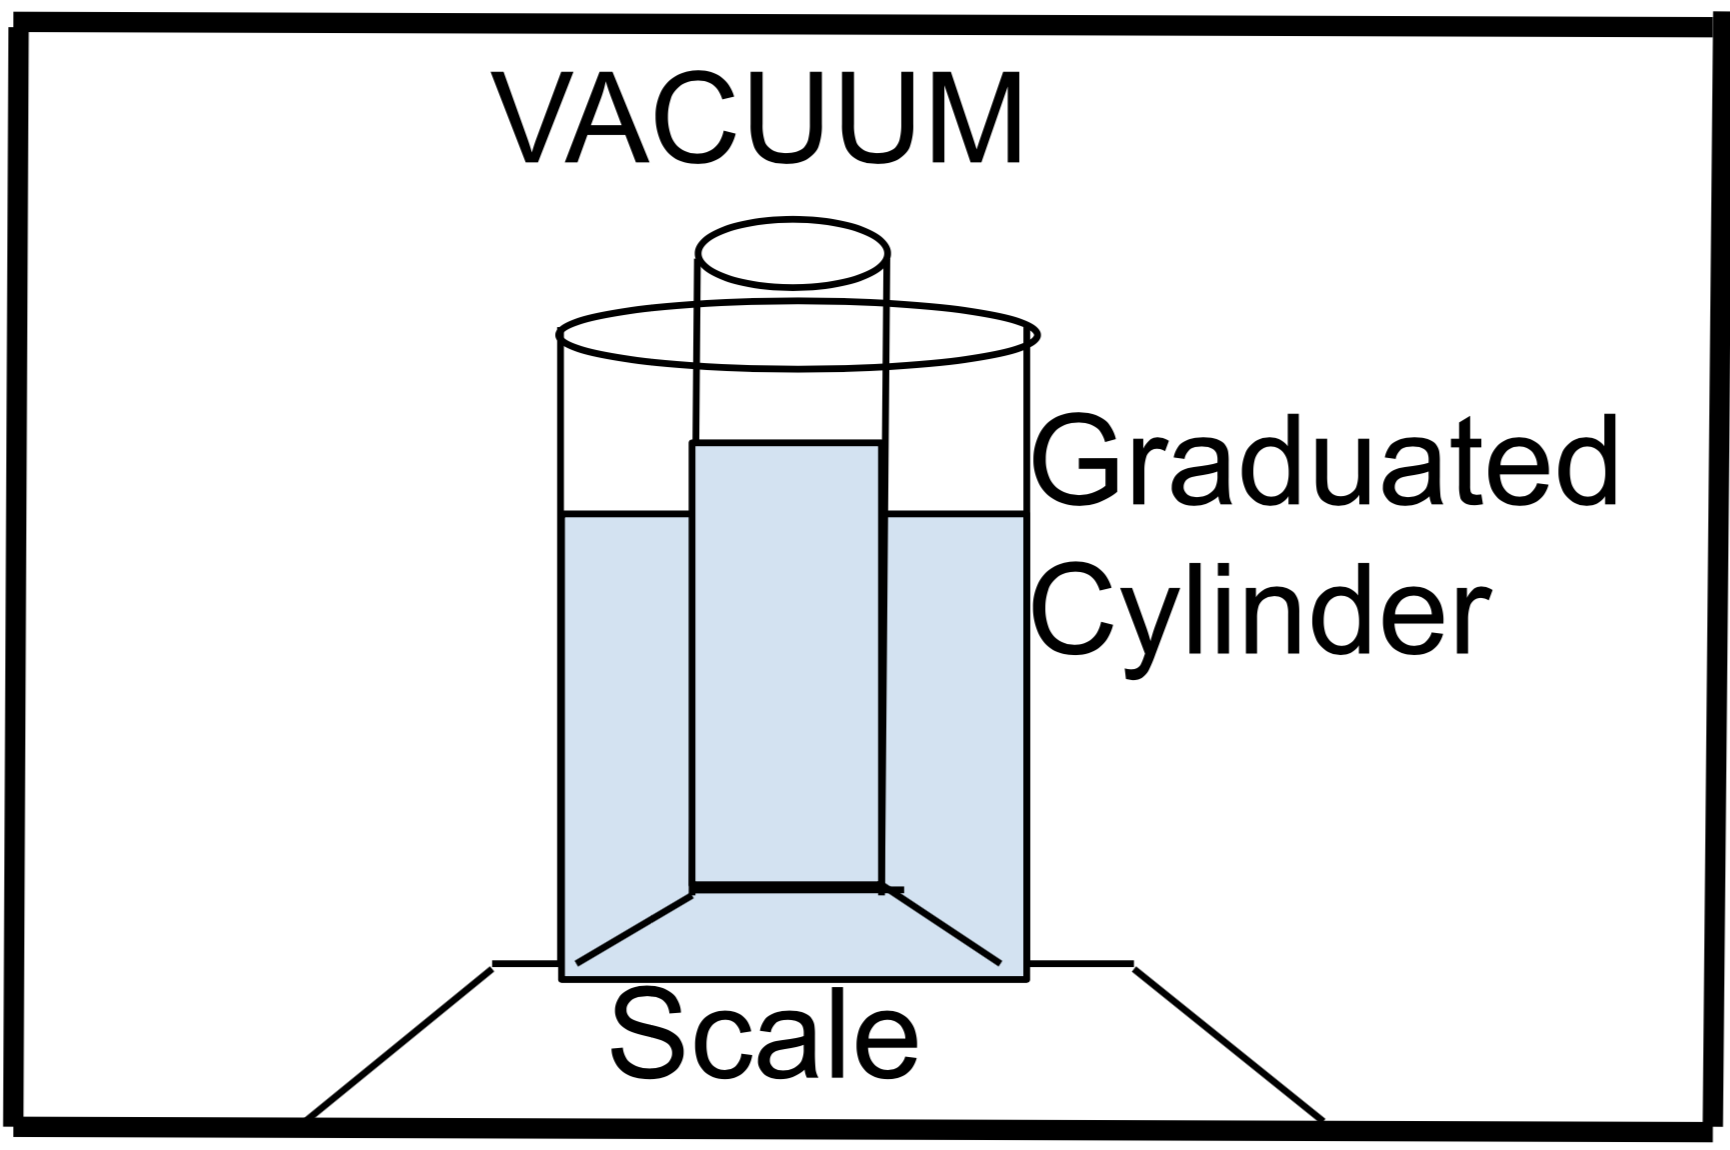
\includegraphics[width = 8cm,height = 6cm]{desinty} 
\end{figure}

Using Eqn x where $m_{LN_{2}}, V_{LN_{2}}$ are the mass loss and volume loss of liquid nitrogen rates and $t$ is the time the experiment was run for. 
\begin{equation}
\rho = \frac{m_{f} - m_{i} + m_{LN_{2}}t} {V_{f} - V_{i} + V_{LN_{2}}t}
\end{equation}

\begin{figure}[h]
 \caption{The phase diagram for nitrogen shows that as the pressure drops, so does the boiling point, thus the liquid remaining is colder than the boiling point at room temperature. }
 \label{NPD}
 \centering
 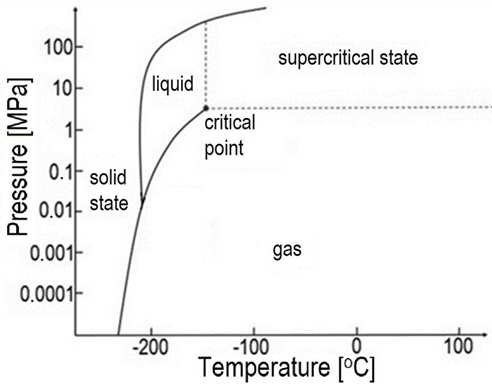
\includegraphics[width = 8cm,height = 6cm]{N_PD} 
\end{figure}





  \section{Results}
  The new procedure for solid ammonia production was used to create a $120$ mL batch of electronics grade solid ammonia in which the material was clear while in the cryostat immediately after being taken off the gas panel. When the slug was submerged in liquid nitrogen it turned an opaque white from all the thermal stress fractures. 
\begin{figure}[h]
 \caption{The material made using coldfinger method. The material made using liquid nitrogen bath. Visual analysis indicates some structural difference. }
 \label{mat}
 \centering
  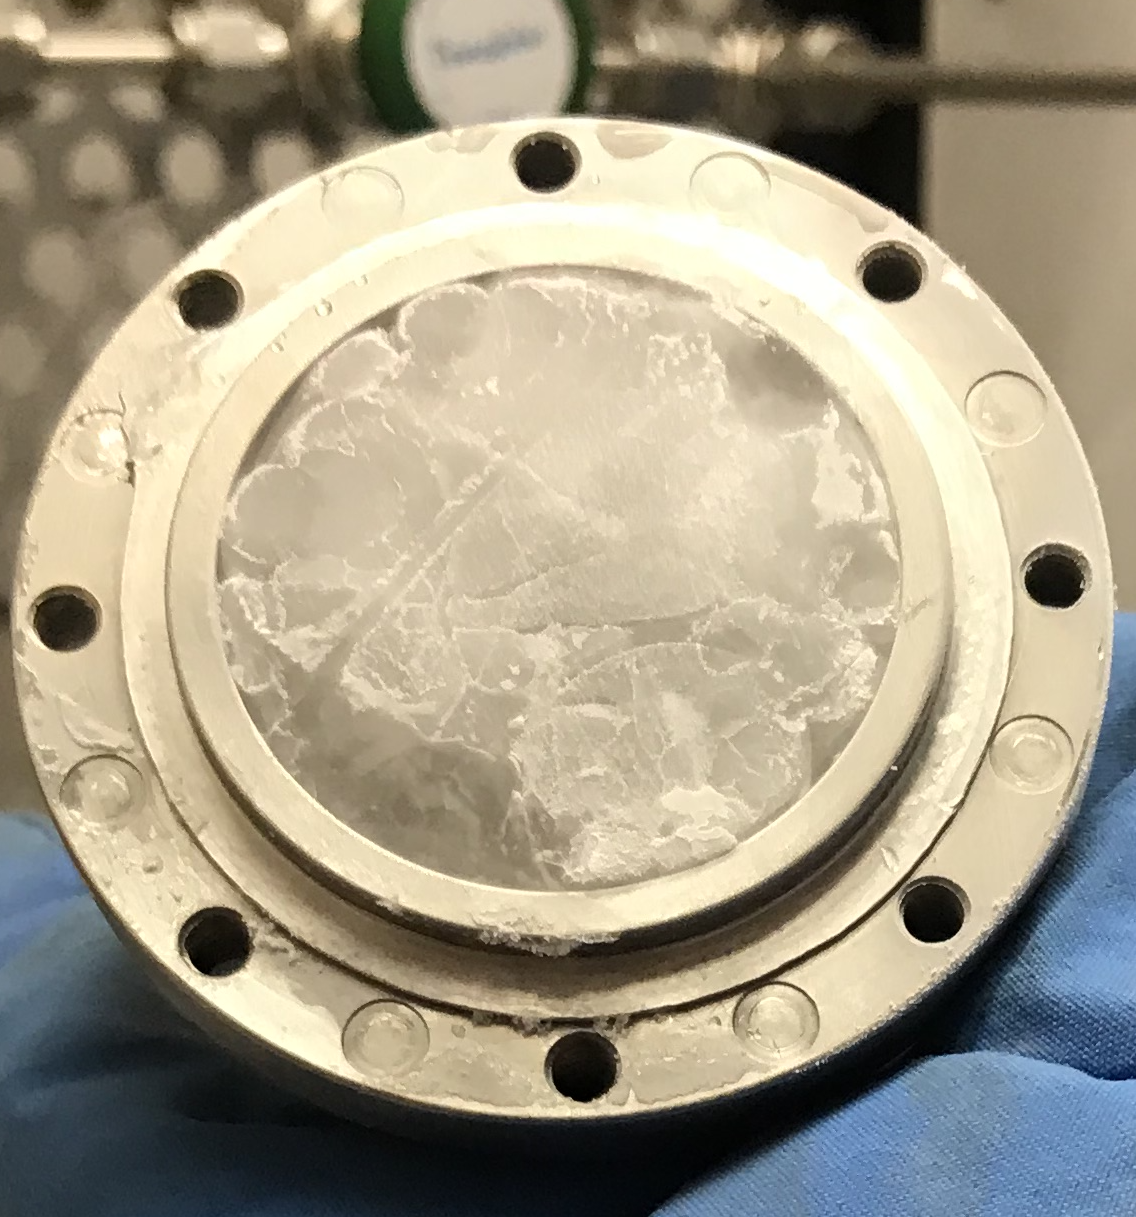
\includegraphics[width = 6cm,height = 6cm]{NH3_CF} 
  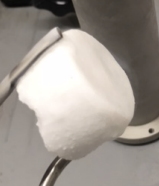
\includegraphics[width = 6cm,height = 6cm]{NH3_LN2} 
\end{figure}

The former process used liquid nitrogen as a cooling bath and with a boiling point of  $77$ K, the interior walls of the cryostat were brought to far below the freezing point of ammonia, $195$ K. This new method uses a coldfinger which acts as a heat sink to bring the temperature of the interior walls to $185$ K, just below the freezing point of ammonia. shown in Figure \ref{Tvt_3}

\begin{figure}[h]
 \caption{lksdagjhabkjsdvads}
 \label{Tvt_3}
 \centering
  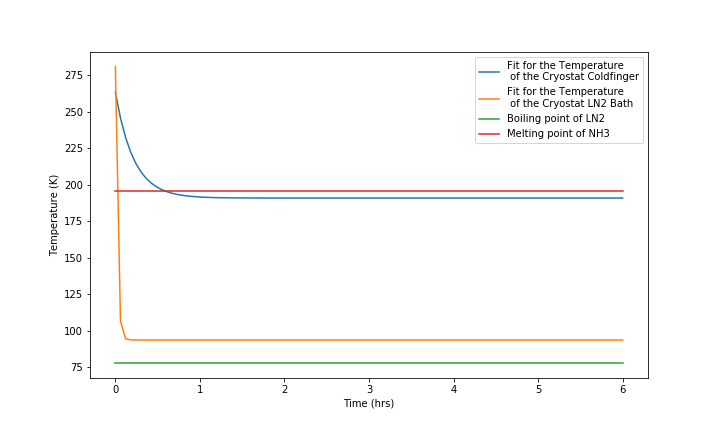
\includegraphics[width = 14cm,height = 8cm]{Temperature_Time_3} 
\end{figure}
The density of a cryogenic solid like solid ammonia can be measured by using a vacuum chamber with a $25$ mL beaker nested in a bath of liquid nitrogen and a scale to measure the mass change. This device shown in Figure \ref{rho}, is still in the testing phase and is yet ready to work with ammonia. 

\begin{center}
\begin{table}[h]
\label{table}
\caption{Obersvations made on the material produced from the different solidification processes. }
\begin{tabular}{|c|c|c|}
\hline
Method & Observation & Operating Temperature \\
\hline
LN$_{2}$ cold bath &  \tabitem White and powdery & $~ 97 $ K \\
&  \tabitem Brittle amorphous solid & \\
\hline
Coldfinger heat sink &  \tabitem Transparent and hard & $~ 185$ K\\
& \tabitem Durable crystalline solid  & \\
\hline
\end{tabular}
\end{table}
\end{center}





\section{Conclusion}
This project was focused on building and implementing a new cooling technique for freezing gaseous ammonia into a solid that is used as a polarized target in scattering experiments. The new method uses a coldfinger heat sink to bring the walls of the cryostat down to a temperature closer to the freezing point of ammonia and allows for a crystalline solid to grow from the bottom. The temperature can be controlled by how much of the coldfinger is submerged in the bath of liquid nitrogen. This needs to be done in order to determine a relation between the level of liquid nitrogen and the internal temperature of the cryostat. Additionally adding in a thermometry display to use as a guide for what the temperature is. By measuring the external temperature of the cryostat a calculation can be made to determine what the internal temperature is and whether that is in the range necessary for solidification. 

\bibliographystyle{plain}
\bibliography{mybib}{}


\newpage









\appendix
\section{Procedure for Solidification of Ammonia using Coldfinger}
  \subsection{Preparation}
      To prepare the cryostat for the freezing of $NH_{3}$ the end-cap and coldfinger must be attached to the bottom. This section will go through the steps needed to prepare the cryostat for freezing $NH_{3}$ safely.
      \begin{enumerate}
          \item Make the Indium seal on the bottom of the cryostat.
            \begin{enumerate}
                \item If the old seal is still on, use small Flathead screwdriver to remove all Indium from the rim of the cryostat. Dispose of waste in Indium Waste tub.
                \item Wipe down both the inside flange of the end-cap and the rim of the cryostat with an acetone soaked kim wipe.
                \item Using wire cutters, cut a $6$ in strand of $99.9\%$ pure Indium.
                \item Wipe the Indium strand down with another  acetone soaked kim wipe.
                \item Wrap the Indium wire around the rim of the cryostat and cross the two ends when the meet. Twist the two ends together to form a knot. Position the knot so that it sits in between the set screw hole and the push screw hole.
                \item Put the cap on and make sure the set screw holes are lined up.
                \item Place the coldfinger on top of the end-cap and begin setting screws (Tighten screws in a star pattern so that the end cap does not get out of level).
            \end{enumerate}
          \item Using a turbo pump, pull vacuum down to $1*10^{-6}$ Torr.
            \begin{enumerate}
                \item Attach the cryostat to the turbo pump using a KF-$25$ clamp and rubber O-ring. Place the O-ring between the KF-$25$ flange of the cryostat and the vacuum tube leading to the pump. Clamp the two together to form vacuum seal.
                \item Make sure the valve to the turbo pump is closed and the vent to atmosphere is open.
                \item Turn on Roughing pump, wait a few minutes then close the vent valve and open the valve to the turbo pump.
                \item Watch pressure drop to $<100$ mTorr.
                \item Turn on the Turbo pump, the pressure on the vacuum gauge will bottom out $(0.00)$ mTorr.
                \item Press the EMS button and watch the pressure drop to about $1*10^{-6}$. The pressure may not get that low but as long as it is in the range of $5*10^{-5}$, it'll be okay. (Add Caution!)
            \end{enumerate}
          \item Attach cryostat to gas panel using a KF-$25$ and rubber O-ring. Place the O-ring between the KF-$25$ flange of the cryostat and the vacuum tube leading to the pump. Clamp the two together to form vacuum seal.
        \end{enumerate}

  \subsection{Solidification}
      The addendum to the process for freezing $NH_{3}$. Prior method involves using $LN_{2}$ as a cold bath and submerging the entire cryostat in the bath to freeze $NH_{3}$. This method uses the a copper heat sink attached to the bottom of the cryostat to draw the heat from the cryostat and dump it in a bath of $LN_{2}$. By keeping the $LN_{2}$ levels steady the bottom of the cryostat will cool down to just below the freezing point of $NH_{3}$. This causes the $NH_{3}$ to liquefy and pool on the bottom and from that a crystal can grow. 
      \begin{enumerate}
      		\item Pump and Purge
      		\begin{enumerate}
      			\item After the cryostat is hooked up verify S$1$ is closed and the NH$_{3}$ bottle valve and regulator valve are closed. 
      			\item Turn on the vacuum pump and open S$2$, S$3$, and V. Verify N and S$1$ is closed.
      			\item Bottom out the analog pressure gauge (~ $-30$ mm Hg) and wait for the digital gauge to get to ~$5$ Torr. 
      			\item Close vacuum and open valve N, wait for the pressure to climb to $9$ PSI (~$465$ Torr).
      			\item Close valve N and open valve V, Bottom out the analog pressure gauge (~ $-30$ mm Hg) and wait for the digital gauge to get to ~$5$ Torr. 
      			\item Repeat steps d - e $3$ times. On the last iteration, leave valve V open for $5$ min. Then close valves S$2$ and V. 
      			\item Turn off the vacuum pump and proceed to step x.x in the manual. 
      		\end{enumerate}
          \item Add $LN_{2}$ to dewar through a full in the $LN_{2}$ port on the dewar after pump/purge.
          \item Allow $~30$ min for coldfinger to cool down before pumping $NH_{3}$
          \item Close S$3$ on the gas panel and begin flowing $NH_{3}$. If pressure does not rise, check the valves
          \item Open S$3$ to flow $NH_{3}$ to cryostat. Over pressurization is normal since the freezing process is so slow.
          \item Keep $LN_{2}$ levels at about $x$ cm (TBD), this ensures the coldfinger is fully submerged
          \item Allow to run for several hours, keeping $LN_{2}$ level constant. $5$ hours yields approximately$120$ mL
          \item After several hours have passed and you want to harvest, close S$1$.
          \item Allow the pressure to come to $150$ Torr or until the pressure does not change in a 15 second window
      \end{enumerate}
%two step freezing process. hold high pressure, low temp, get all liquid. Then submerge in cold bath at 195 K 
\end{document}



